\begin{frame}{Introduction}

\begin{exampleblock}{Données}
\begin{itemize}
\item Matrice de signal $X \in \mathbb{R}^{n \times p}$
\item $n$ observations dans le temps, 1 par image
\item $p$ caractéristiques extraites des images
\end{itemize}
\end{exampleblock}

\begin{block}{Objectif}
Déterminer les ruptures dans la vidéo au travers des caractéristiques extraites, dont la distribution est supposée stationnaire pour une séquence donnée.
\end{block}

\end{frame}

\begin{frame}{Prétraitement des caractéristiques}

{
\definecolor{tempGreen}{HTML}{96EAC0}
\setbeamercolor{block body example}{use=structure,fg=black,bg=tempGreen}
\begin{exampleblock}{Caractéristiques obtenues}
\centering
\includegraphics<1>[width=\textwidth]{images/signal}
\includegraphics<2>[width=.6\textwidth]{images/signal}
\end{exampleblock}
}

\begin{alertblock}<2>{Remarque}
	Peu de valeurs éloignées de 0 \\
	$\Rightarrow$ Prétraitement de la matrice de caractéristiques
\end{alertblock}
\end{frame}

\begin{frame}{Prétraitement des caractéristiques}{Résultat}

{
\definecolor{tempGreen}{HTML}{96EAC0}
\setbeamercolor{block body example}{use=structure,fg=black,bg=tempGreen}
\begin{exampleblock}{Caractéristiques après prétraitement ($\log (10^9 X + 1)$)}
\centering
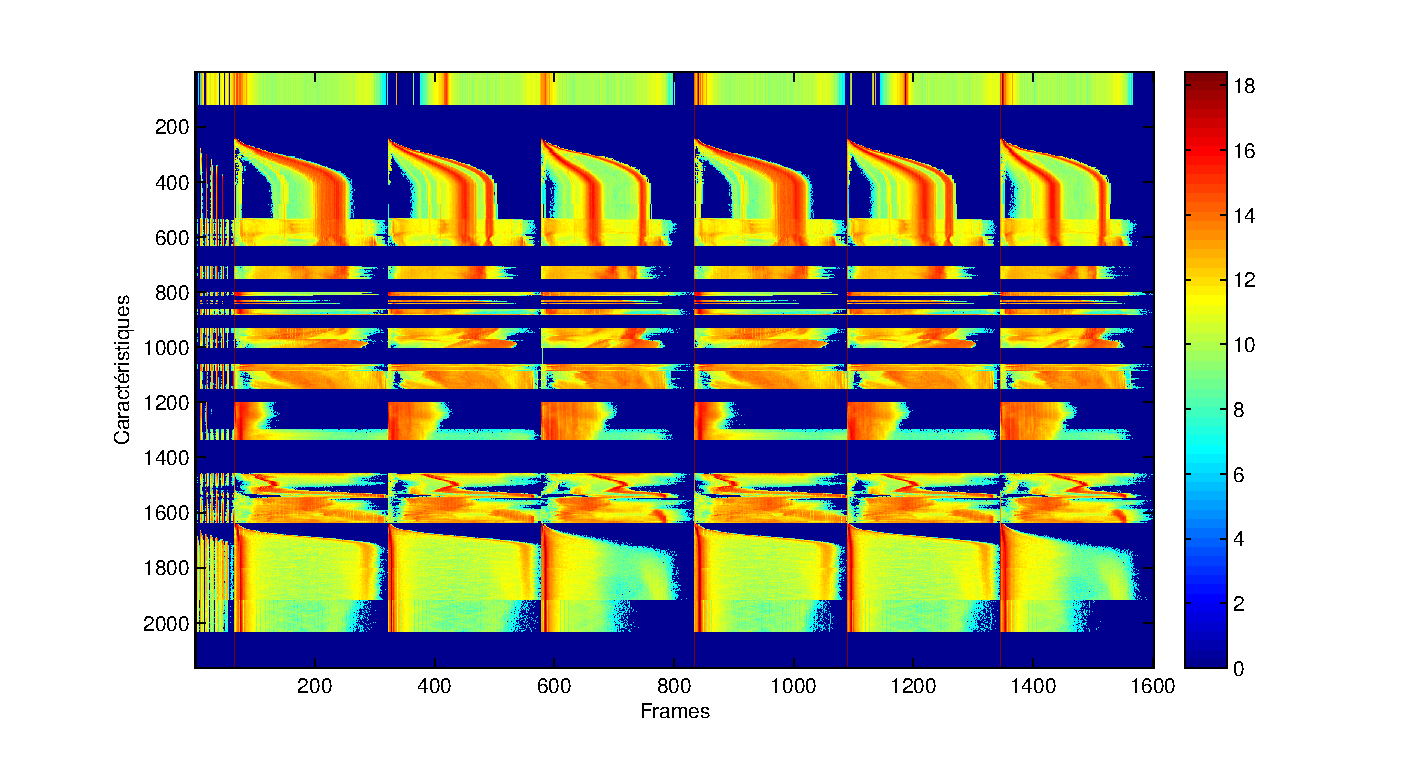
\includegraphics[width=\textwidth]{images/signalPreprocessed}
\end{exampleblock}
}

\end{frame}


\begin{frame}{Méthodes essayées}

\begin{alertblock}{Méthodes essayées}
\begin{itemize}
\item Méthode par dérivée filtrée utilisant la $p$-valeur\\
\textit{Source : \cite{Bertrand11} et \cite{Herault14}}
\item Méthode de détection de changement de noyau\\
\textit{Source : \cite{Desobry05}}
\end{itemize}
\end{alertblock}

\end{frame}


\begin{frame}{Dérivée filtrée}{Principe}

\begin{center}
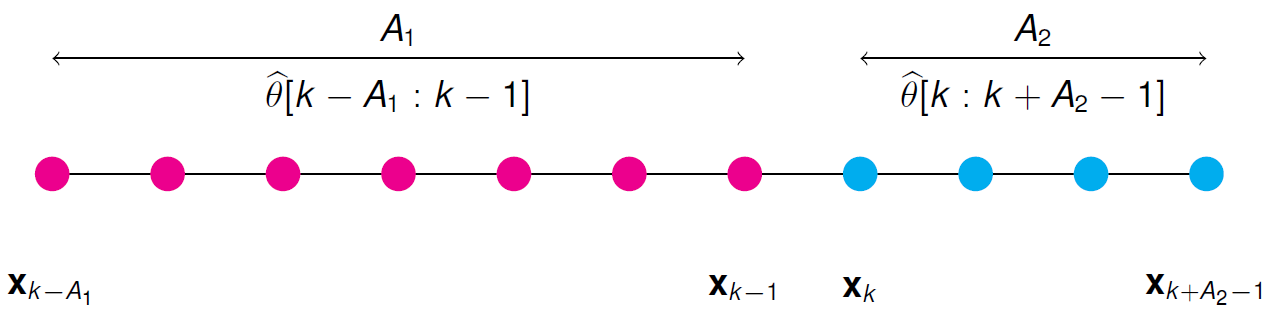
\includegraphics[width=0.8\textwidth]{images/deriveeFiltree}
\end{center}

\begin{block}{Principe}
\begin{itemize}
\item Parcours du signal avec deux fenêtre de taille $A_1$ et $A_2$
\item Distance $D(k)$ entre indicateurs $\hat{\theta}$ sur chaque fenêtre
\item Zones de rupture $\mathcal{K}_i = \{k \text{ successifs t.q. } |D(k)| > C\}$
\item Rupture en $k_{r_i} = \displaystyle \argmax_{k \in \mathcal{K}_i} |D(k)| \hspace{1em}\forall i$
\end{itemize}
\end{block}


\end{frame}

\begin{frame}{Dérivée filtrée}{Détermination de $C$}

\begin{block}{Principe probabiliste basée sur la $p$-valeur}
\vspace{-.7em}
\begin{itemize}
\item Hypothèse $\mathcal{H}_0$ : il n'y a pas de rupture
\item $M = \displaystyle \max_{k} |D(k)|$
\item On veut $C$ tel que $\mathbb{P}(M>C\mid	\mathcal{H}_0) < p$ avec $p$ fixé
\end{itemize}
\end{block}

\begin{exampleblock}{Méthode d'estimation de $C$}
\vspace{-.7em}
\begin{itemize}
\item Création de $\{X_{\mathcal{H}_0}\} = \{\randperm{(X)}\}$ données sous $\mathcal{H}_0$
\item Estimation de $\{M_{\mathcal{H}_0}\}$ sur ces données
\item Estimation de la distribution de $M$ sous $\mathcal{H}_0$
\item Estimation de $C$ tel que $\mathbb{P}(M>C\mid	\mathcal{H}_0) < p$
\end{itemize}
\end{exampleblock}

\end{frame}

\begin{frame}{Changement de noyau}{Principe}

\begin{block}{Principe}
\vspace{-.7em}
\begin{itemize}
\item Cas particulier de la dérivée filtrée
\item Indicateurs $\hat{\theta}$ étant les paramètres d'un \textit{one-class SVM} sur chaque fenêtre
\item Mesure de distance particulière entre les kernels
\end{itemize}
\end{block}

\end{frame}

\begin{frame}{Changement de noyau}{Distance}

\begin{columns}
\begin{column}{.47\textwidth}
\small
\begin{align}
  D &= \frac{\overset{\frown}{c_1 c_2}}{\overset{\frown}{c_1 p_1} + \overset{\frown}{c_2 p_2}} \notag \\
  \overset{\frown}{c_1 c_2} &= \arccos\left(\frac{
    	\langle w_1, w_2\rangle_\mathcal{H}
    	}{
    	\|w_1\|_\mathcal{H}\|w_2\|_\mathcal{H}
    	} \right) \notag \\
   &= \arccos\left(\frac{
  	\alpha_1^\top K_{12} \alpha_2
  	}{
  	\sqrt{\alpha_1^\top K_{11} \alpha_1} \sqrt{\alpha_2^\top K_{22} \alpha_2}
  	} \right) \notag \\
  \overset{\frown}{c_i p_i} &= \arccos\left( \frac{\rho_i}{\sqrt{\alpha_i^\top K_{ii} \alpha_i}}  \right) \notag
\end{align}

~\\~\\
$i, j = 1$ pour les données avant $k$ et $2$ pour les données après.

\end{column}
\begin{column}{.47\textwidth}

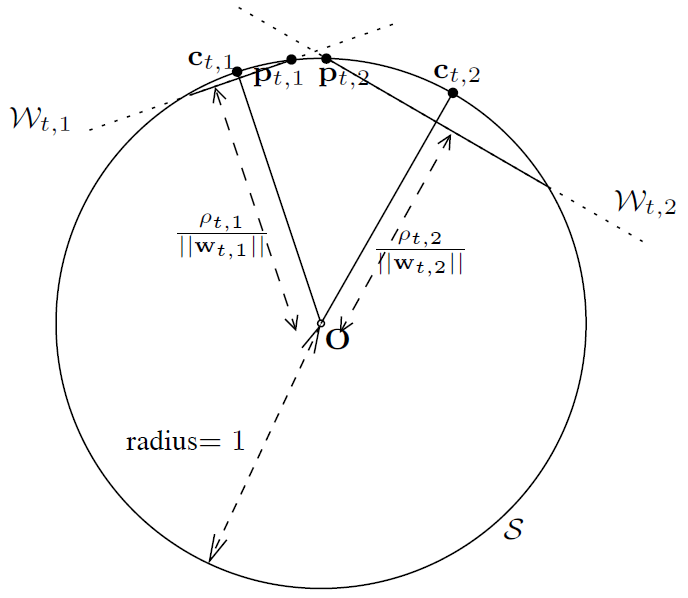
\includegraphics[width=\textwidth]{images/svm}


\begin{itemize}
\item $\alpha_i$ : variables duales
\item $w_i$ : poids de l'hyperplan
\item $\rho_i$ : biais de l'hyperplan
\item $K_{ij}$ : matrice de Gram
\end{itemize}

\end{column}
\end{columns}

\end{frame}

\begin{frame}{Détermination des paramètres $A_i, C$}

\begin{block}{Détermination des paramètres $A_i, C$}
\begin{itemize}
\item Détermination de $A_1$ en essayant différentes valeurs et en visualisant $D$ ($A_2=A_1$).
\item Détermination de $A_2$ en essayant différentes valeurs et en visualisant $D$.
\item Détermination de $C$ visuellement.\\
\textit{Très mauvais résultats avec la méthode de la $p$-valeur avec 200 tirages aléatoires.}
\end{itemize}
\end{block}

\end{frame}

\begin{frame}{Résultat final}{Différence de moyennes}

{
\definecolor{tempGreen}{HTML}{96EAC0}
\setbeamercolor{block body example}{use=structure,fg=black,bg=tempGreen}
\begin{exampleblock}{Distance et ruptures détectées, $A_1 = 20, A_2 = 28, C = 0,6$}
\centering
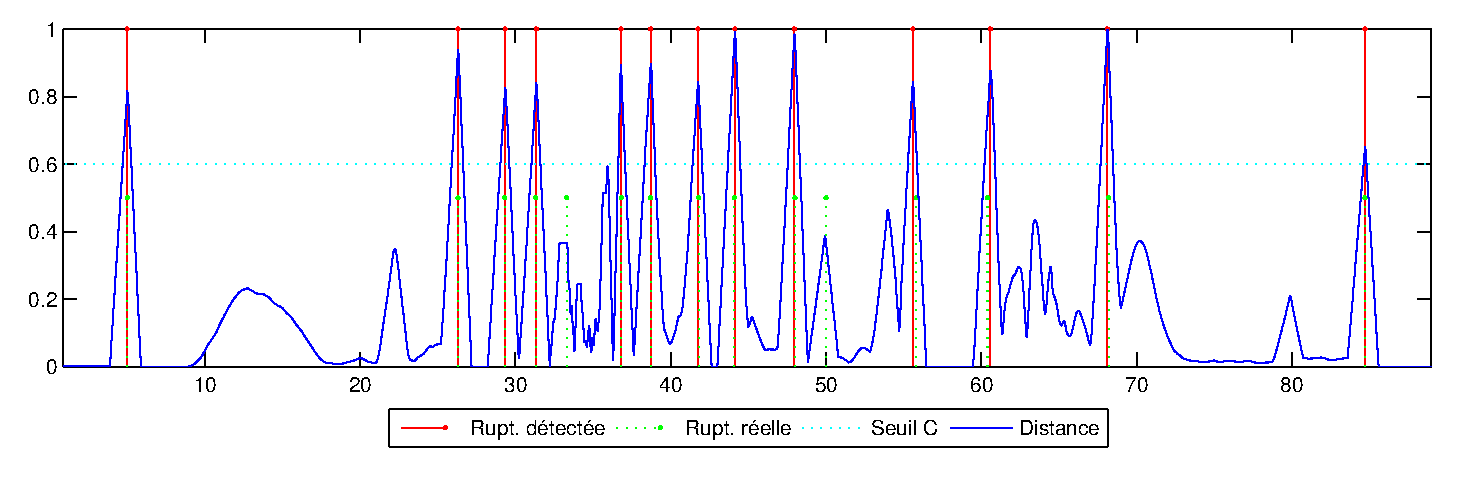
\includegraphics[width=\textwidth]{images/resultatMoy}
\end{exampleblock}
}

\end{frame}

\begin{frame}{Résultat final}{Distance \textit{one-class SVM}}

{
\definecolor{tempGreen}{HTML}{96EAC0}
\setbeamercolor{block body example}{use=structure,fg=black,bg=tempGreen}
\begin{exampleblock}{Distance et ruptures détectées, $A_1 = 20, A_2 = 28, C = 0,8$}
\centering
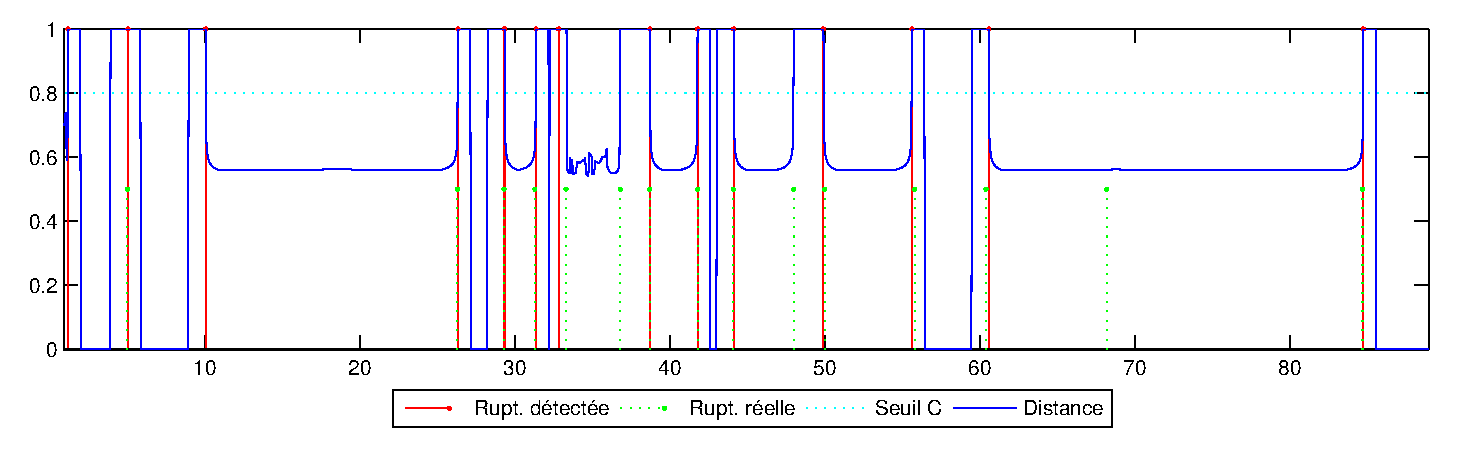
\includegraphics[width=\textwidth]{images/resultatSVM}
\end{exampleblock}
}

\end{frame}
